\documentclass[table]{beamer}

\usepackage{subfigure}
\usepackage{amssymb}
\usepackage{amsmath}
\usepackage{epsfig}

\usepackage{longtable}

\usepackage{url}
\usepackage[polish]{babel}
\usepackage[utf8]{inputenc}
\usepackage[T1]{fontenc}
% \usetheme{Warsaw}
% \usetheme{Frankfurt}
\usetheme{boxes}
% \usecolortheme{seahorse}
% \renewcommand{\inserttotalframenumber}{18}
% \setbeamertemplate{footline}[page number]

\title{Systematyczne przetwarzanie informacji o rearanżacjach genomowych w R}
\author{Piotr Dittwald (MISDoMP/MIMUW)}
\institute{piotr.dittwald@gmail.com}
%\titlegraphic{\includegraphics[width=1.2cm]{images/uwlogo.png}}
\date{SER IV, Warszawa, \small{22 V 2014}}


\begin{document}

\begin{frame}
  \titlepage
%  \includegraphics[width=1.7cm]{dit_pic/uwlogo.png}
% \includegraphics[width=2.7cm]{dit_pic/mimuwlogo.png}
\end{frame}

\begin{frame}
\frametitle{Czego można się spodziewać?}
\begin{itemize}
\item Motywacje biologiczne
\item Analiza bioinformatyczna
\item Kod w R
\end{itemize}
\end{frame}


\begin{frame}\frametitle{Ludzki genom}
 \begin{columns}
    \column{0.5\textwidth}
	    \begin{center}
	   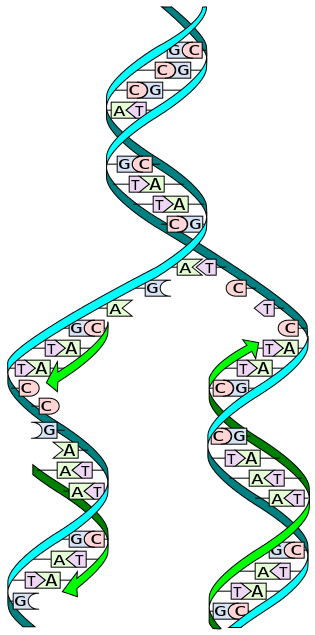
\includegraphics[width=0.6 \textwidth]{SER-images/DNA_replication.png}\\
	   \tiny{źródło: wikipedia}  
	    \end{center}
    \column{0.5\textwidth}
\begin{itemize}
\item cztery możliwe nukleotydy: adenina (A), cytozyna (C), tymina (T), guanina (G)
\item dwie helisy DNA
\item komplementarne pary nukleotydów: A-T, G-C 
\end{itemize}
\end{columns}
\end{frame}

\begin{frame}\frametitle{Kariotyp}
 \begin{columns}    
    \column{0.5\textwidth}
\begin{itemize}
\item chromosomy 1-22
\item chromosomy płciowe
\begin{itemize}
\item mężczyzna: X-Y
\item kobieta: X-X
\end{itemize}
\end{itemize}
 \column{0.5\textwidth}
	    \begin{center}
	   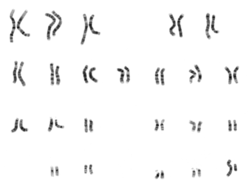
\includegraphics[width=0.9 \textwidth]{SER-images/karyotype.png}\\
	   \tiny{źródło: wikipedia}  
	    \end{center}
\end{columns}
\end{frame}


\begin{frame}\frametitle{Chromosomy bliżej}
 \begin{columns}    
 \column{0.5\textwidth}
\begin{itemize}
\item ramiona p i q
\item centromer
\item prążki widoczne po zabarwieniu barwnikiem
\end{itemize}

 \column{0.5\textwidth}
	    \begin{center}
	   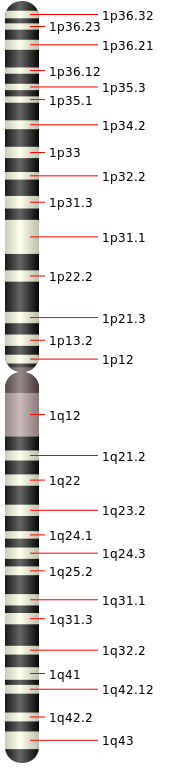
\includegraphics[width=0.3 \textwidth]{SER-images/Chromosome_1.png}\\
	   \tiny{źródło: http://ghr.nlm.nih.gov/chromosome=1}  
	    \end{center}
\end{columns}
\end{frame}


\begin{frame}\frametitle{Geny}
 \begin{columns}    
\column{0.5\textwidth}
	    \begin{center}
	   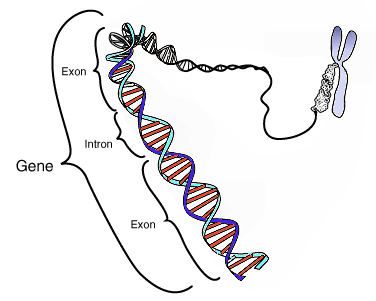
\includegraphics[width=0.9 \textwidth]{SER-images/Gene.png}\\
	   \tiny{źródło: wikipedia}  
	    \end{center}
 \column{0.5\textwidth}
\begin{itemize}
\item będziemy je traktowali jako przedziały na genomie
\item często są powiązane z chorobami (np. baza danych OMIM.org)
\end{itemize}
\end{columns}
\end{frame}


\begin{frame}\frametitle{Bioconductor.org}  
\begin{itemize}  
 \item repozytorium pakietów do bioinformatyki
 \item na stronie dostępna dokumentacja i tzw. {\em vignette}
\end{itemize}
\begin{center}
	   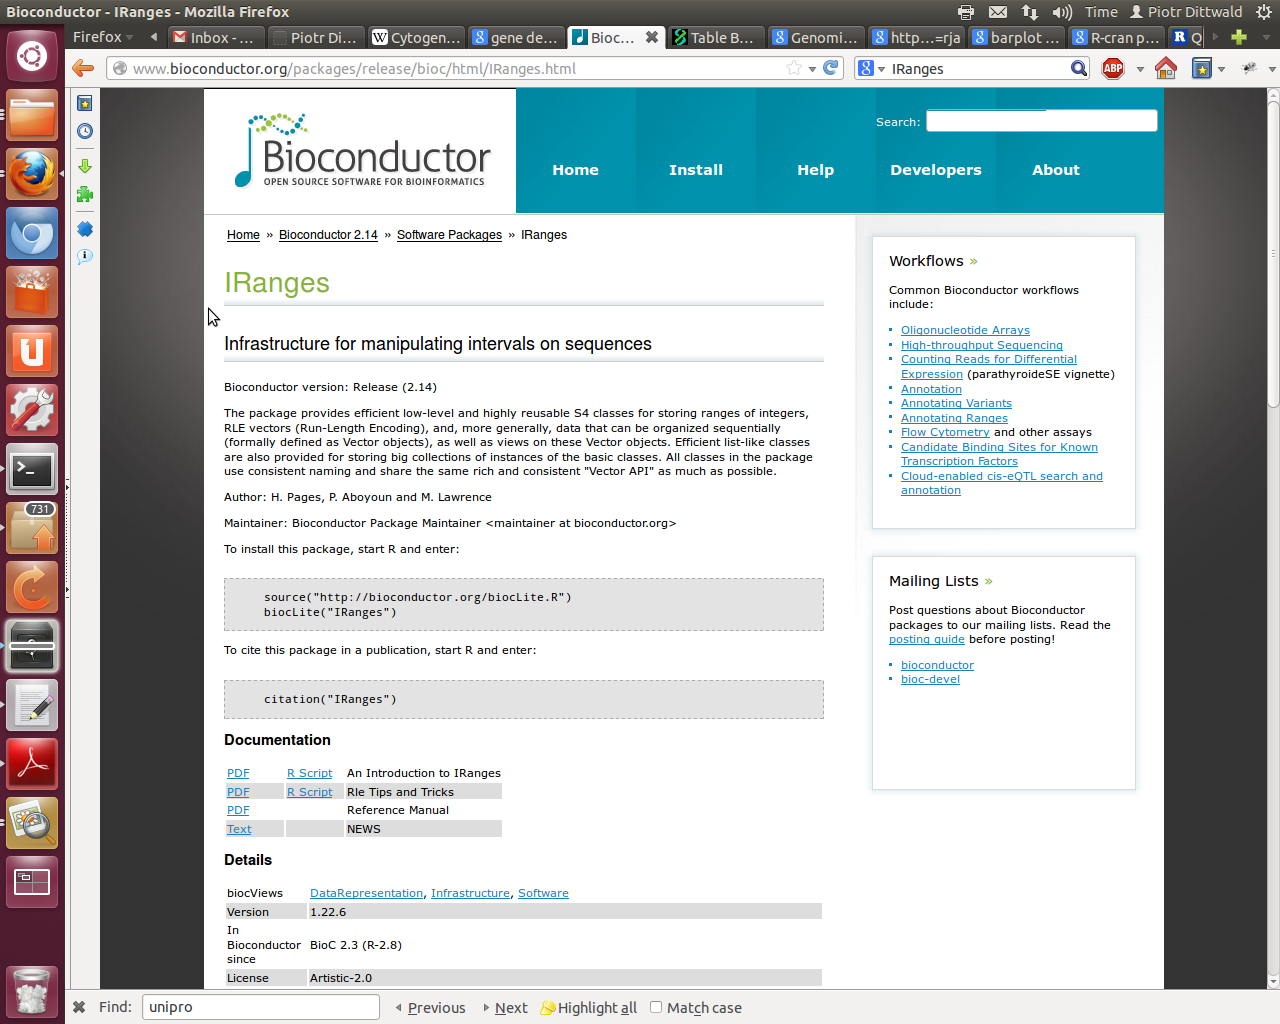
\includegraphics[width=0.9 \textwidth]{SER-images/Bioconductor.png}\\	   
	    \end{center}
\end{frame}


\begin{frame}\frametitle{Źródło danych - przeglądarka UCSC}  
\begin{itemize}  
 \item zbiory danych: 
\begin{itemize}
	\item do oglądania w przeglądarce
	\item do ściągnięcia przez Table Browser
\end{itemize}
 \item np. RefSeq, UCSC Genes
\end{itemize}
\begin{center}
	   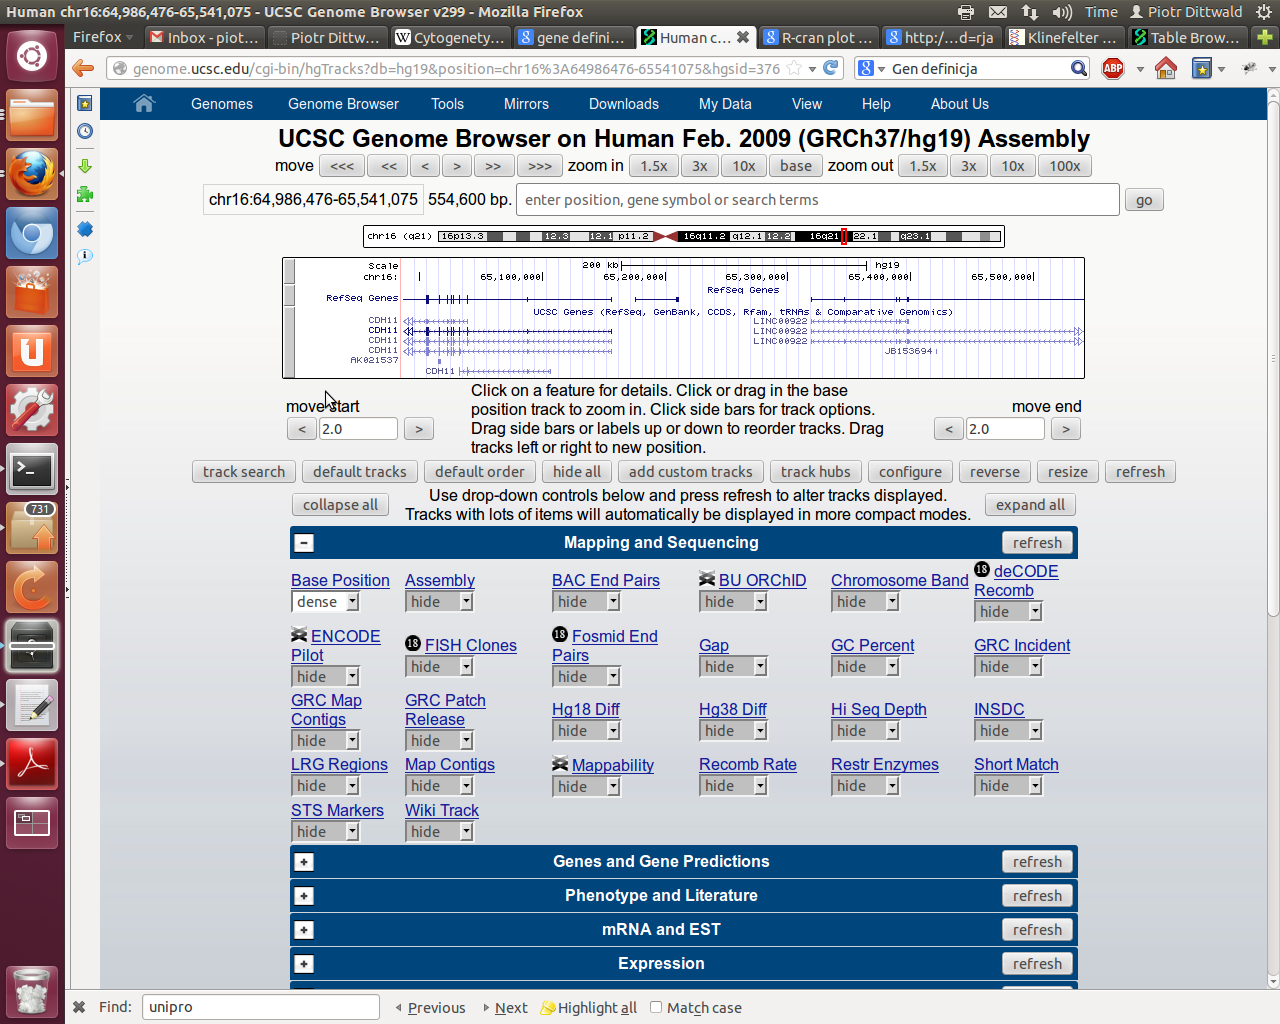
\includegraphics[width=0.9 \textwidth]{SER-images/UCSC.png}\\	   
	    \end{center}
\end{frame}

\begin{frame}\frametitle{Aberracje chromosomowe}
 \begin{columns}    
    \column{0.5\textwidth}
 Syndrom Klinefeltera
 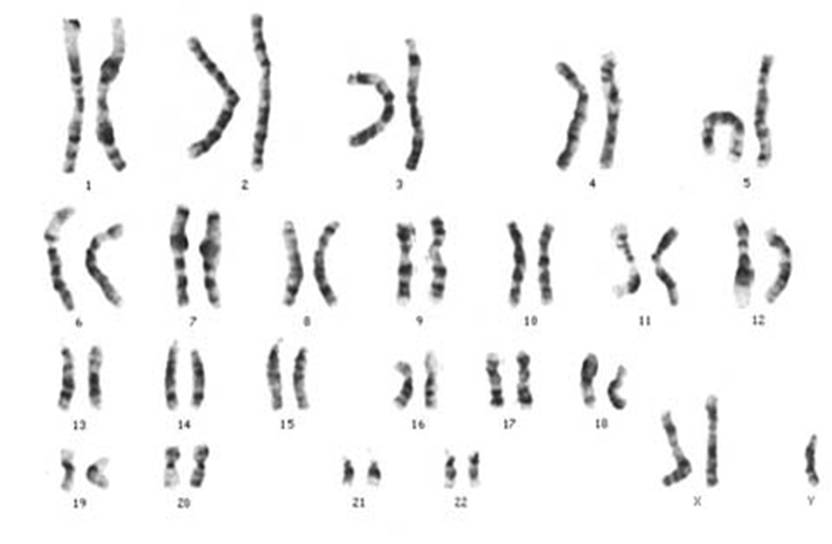
\includegraphics[width=0.9 \textwidth]{SER-images/Klinefelter_syndrome_kariotyp.jpg}\\
	   \tiny{źródło: wikipedia}  

 \column{0.5\textwidth}
 Syndrom Downa
    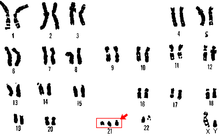
\includegraphics[width=0.9 \textwidth]{SER-images/Down_syndrome_karyotype.png}\\
	   \tiny{źródło: wikipedia}  	    
\end{columns}
\end{frame}


\begin{frame}\frametitle{CNVs}
\begin{columns}    
    \column{0.5\textwidth}
\begin{center}
	   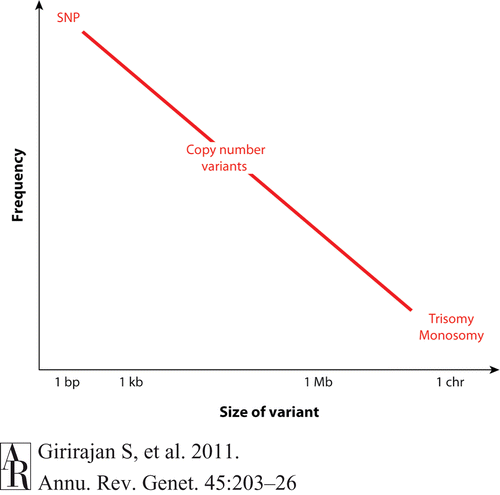
\includegraphics[width=0.9 \textwidth]{new-images/CNVsize.png}\\
\end{center}
 \column{0.5\textwidth}
\begin{itemize}
\item obszary genomu, których u danego osobnika jest mniej lub wiecej niż w referencyjnym genomie,
nazywamy wariantami o zmienionej liczbie kopii ({\em ang. Copy-Number Variants; CNVs})
\item w szczególności CNVs występują między długimi (10-400 kb) fragmentami DNA o wysokim ($>$ 97\%) współczynniku podobienstwa sekwencyjnego (mechanizm NAHR)
\end{itemize}
\end{columns}
\end{frame}


\begin{frame}\frametitle{Geny recesywne na chromosomie X}
	    \begin{center}
	   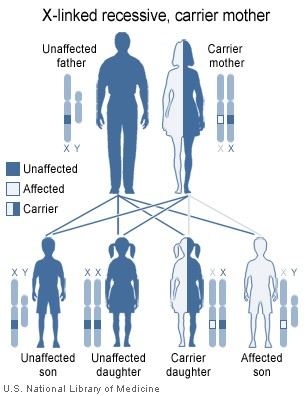
\includegraphics[width=0.5 \textwidth]{new-images/XlinkRecessive.jpg}\\
	   \tiny{źródło: wikipedia}  
	    \end{center}
\end{frame}

\begin{frame}\frametitle{Dane kliniczne}
 \begin{columns}   
    \column{0.5\textwidth}
	    \begin{center}
	   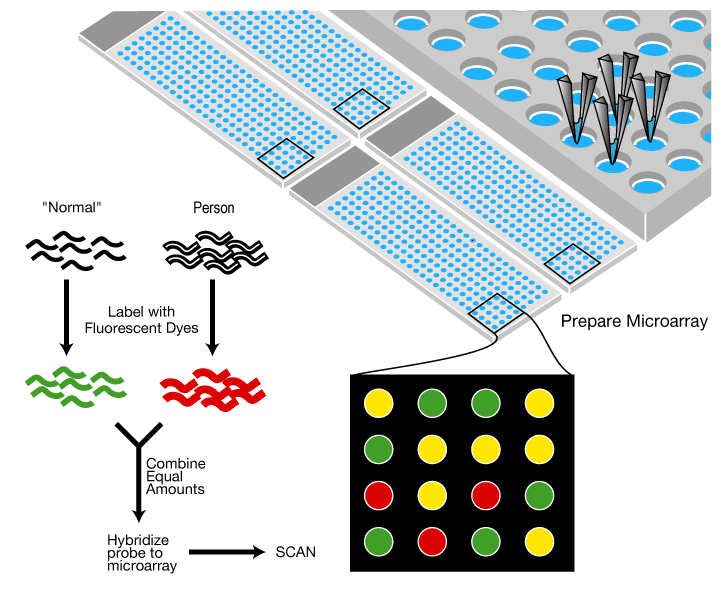
\includegraphics[width=\textwidth]{new-images/hybridization.png}\\
	   \tiny{source: atlantichealth.dnadirect.com}  
	    \end{center}
   \column{0.5\textwidth}
  \begin{itemize}
  \item metoda porównawczej hybrydyzacji genomowej do mikromacierzy ({\em ang. microarray-based Comparative
Genomic Hybridization; aCGH})
  \item dane kliniczne $> 25,000$ pacjentów z bazy Baylor College of Medicine, Houston
 \end{itemize}
\end{columns}
   
\end{frame}

% 
% 
% \begin{frame}
% \frametitle{Collaboration}  
% \small{
% Anna Gambin$^a$, J\"{u}rgen Claesen $^b$, Tomasz Burzykowski $^b$, Dirk Valkenborg $^{b,c, d}$\\
% $a:$ University of Warsaw, Poland\\
% $b:$ Hasselt University, Belgium\\
% $c:$ Flemish Institute for Technological Research (VITO), Belgium\\
% $d:$ CfP-CeProMa, University of Antwerp, Belgium\\
% }
% 
%\underline{Piotr Dittwald}, Tomasz Gambin, Claudia Gonzaga-Jauregui, Claudia M.B. Carvalho, James R. Lupski, Paweł Stankiewicz, Anna Gambin


% \begin{block}{}
% The research was in part supported by the EU through the European Social Fund, contract number UDA-POKL.04.01.01-00-072/09-00. 
% \end{block}
% 
%  
% \end{frame}
% 
% 
% 
% 
% % 
% % 
% \begin{frame}
% \frametitle{Bibliography}  
% \begin{thebibliography}{}
% % \begin{tiny}
% 
% \bibitem[Claesen et al.]{claesen} Claesen J., Dittwald P., Burzykowski T., and Valkenborg D. \\An efficient method to calculate the aggregated isotopic
% distribution and exact center-masses, \textit{accepted to Journal of The American Society for Mass Spectrometry}. to appear in 2012
% \bibitem[]{}Valkenborg, D., Mertens, I., Lemière, F., Witters, E. and Burzykowski, T. 2011, The isotopic distribution conundrum. Mass Spectrometry Reviews, 30: n/a. \\doi: 10.1002/mas.20339. 
% \bibitem[]{}Macdonald I.G., Symmetric functions and Hall polynomials / by I. G. Macdonald. Clarendon Press; Oxford University Press, Oxford : New York, 1979.
% % \end{tiny}
% \end{thebibliography}
% 
% \end{frame}
% % 
% \appendix
% 
% \begin{frame}
% \begin{center}
%  \Huge{Thank you!}
% \end{center}
%  \end{frame}
\end{document}
